\documentclass[12pt]{article}

\usepackage{amsmath}
\usepackage{amsthm}
\usepackage{fancyhdr}
\pagestyle{plain}
\usepackage{tikz}
\usepackage{float}

\tikzset{node distance=2.5cm, auto}

\author{Evgeny Kotelnikov}
\title{Exercises for Chapter 1}
\date{}

\begin{document}
\maketitle

\begin{enumerate}
  \item[1.]
    In order to show that $\mathbf{Rel}$ is a category we need to prove associativity and unit laws.

    \newtheorem*{assoc}{Associativity law}
    \begin{assoc}
      $$h \circ (g \circ f) = (h \circ g) \circ f$$ for all $f \subseteq A \times B$, $g \subseteq B \times C$ and $h \subseteq C \times D$.
    \end{assoc}

    \begin{proof}
      \begin{equation*}
        \begin{array}{rl}
          h \circ (g \circ f) & = \{\langle a, d\rangle \in A \times D~|~\exists\, c~(\langle a, c \rangle \in g \circ f~\&~\langle c, d \rangle \in h) \} \\
                              & = \{\langle a, d\rangle \in A \times D~|~\exists\, c, b~(\langle a, b \rangle \in f~\&~\langle b, c \rangle \in g~\&~\langle c, d \rangle \in h) \} \\
                              & = \{\langle a, d\rangle \in A \times D~|~\exists\, b~(\langle a, b \rangle \in f~\&~\langle b, d \rangle \in h \circ g) \} \\
                              & = (h \circ g) \circ f.
        \end{array}
      \end{equation*}
    \end{proof}

    \newtheorem*{unit}{Unit law}
    \begin{unit}
      $$f \circ 1_A = f = 1_B \circ f$$ for all $f \subseteq A \times B$.
    \end{unit}

    \begin{proof}
      \begin{equation*}
        \begin{array}{rl}
          f \circ 1_A & = \{\langle a, b \rangle \in A \times B~|~\exists\, x~(\langle a, x \rangle \in 1_A~\&~\langle x, b \rangle \in f)\} \\
                      & = [\langle a, x \rangle \in 1_A \Rightarrow x = a] \\
                      & = \{\langle a, b \rangle \in f\} \\
                      & = f.
        \end{array}
      \end{equation*}
      \begin{equation*}
        \begin{array}{rl}
          1_B \circ f & = \{\langle a, b \rangle \in A \times B~|~\exists\, x~(\langle a, x \rangle \in f~\&~\langle x, b \rangle \in 1_B)\} \\
                      & = [\langle x, b \rangle \in 1_B \Rightarrow x = b] \\
                      & = \{\langle a, b \rangle \in f\} \\
                      & = f.
        \end{array}
      \end{equation*}
    \end{proof}

  \item[10.]
    Let's calculate the number of all the possible free categories with 6 arrows, enumerating the number of possible vertices and edges in underlying directed graph and summing results along the way.
    \begin{enumerate}
      \item Free category with one object $A$ only has one morphism $1_A$.
      \item Free category with two objects $A$ and $B$ has identity morphisms $1_A$ and $1_B$ by default. We are looking for a graph, that produces exactly four more arrows. If a graph has exactly one edge, that will produce exactly one arrow, which isn't enough. If a graph has exactly two edges, then they are either parallel, or form a loop. In the first case that will produce only two arrows. In the second case it will form infinite number of finite paths and infinite number of arrows in a category. Therefore we cannot have loops in a graph. Three edges is not enough either. The only possible option is a graph, that has four edges pointing in the same direction.
            \begin{figure}[H]
              \centering
              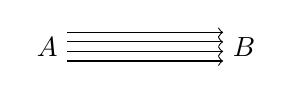
\begin{tikzpicture}
                \node (A)              {$A$};
                \node (B) [right of=A] {$B$};
                \draw[->,transform canvas={yshift=0.4ex}]  (A) to node {} (B);
                \draw[->,transform canvas={yshift=-0.4ex}] (A) to node {} (B);
                \draw[->,transform canvas={yshift=1.2ex}]  (A) to node {} (B);
                \draw[->,transform canvas={yshift=-1.2ex}] (A) to node {} (B);
              \end{tikzpicture}
            \end{figure}
            Category with arrows pointing from $B$ to $A$ is isomorphic to this one, so we don't count it twice.
      \item Free category with three objects $A$, $B$ and $C$ hac three identity morphisms $1_A$, $1_B$ and $1_C$ by default. We are looking for a graph, that produces exactly three more arrows. If the graph has one edge, that will produce exactly one more arrow. If the graph has two arrows, that will produce two arrows. The only combination of edges, that form strictly one path by concatenation is the following one.
            \begin{figure}[H]
              \centering
              \begin{tikzpicture}
                \node (A)              {$A$};
                \node (B) [right of=A] {$B$};
                \node (C) [right of=B] {$C$};
                \draw[->] (A) to node {} (B);
                \draw[->] (B) to node {} (C);
              \end{tikzpicture}
            \end{figure}
            If the graph has three arrows, it produces three arrow. At the same time, they should not form any paths, so we willn't ended up with more arrows, that it, no edge's source should de some other edge's target. That yields three more graphs.
            \begin{figure}[H]
              \centering
              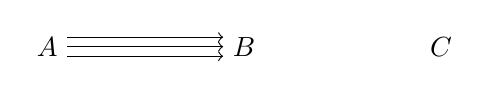
\begin{tikzpicture}
                \node (A)              {$A$};
                \node (B) [right of=A] {$B$};
                \node (C) [right of=B] {$C$};
                \draw[->] (A) to node {} (B);
                \draw[->,transform canvas={yshift=0.8ex}]  (A) to node {} (B);
                \draw[->,transform canvas={yshift=-0.8ex}] (A) to node {} (B);
              \end{tikzpicture}
            \end{figure}
            \begin{figure}[H]
              \centering
              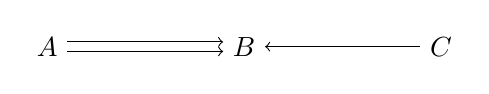
\begin{tikzpicture}
                \node (A)              {$A$};
                \node (B) [right of=A] {$B$};
                \node (C) [right of=B] {$C$};
                \draw[->,transform canvas={yshift=0.4ex}]  (A) to node {} (B);
                \draw[->,transform canvas={yshift=-0.4ex}] (A) to node {} (B);
                \draw[->] (C) to node {} (B);
              \end{tikzpicture}
            \end{figure}
            \begin{figure}[H]
              \centering
              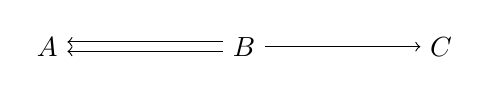
\begin{tikzpicture}
                \node (A)              {$A$};
                \node (B) [right of=A] {$B$};
                \node (C) [right of=B] {$C$};
                \draw[->,transform canvas={yshift=0.4ex}]  (B) to node {} (A);
                \draw[->,transform canvas={yshift=-0.4ex}] (B) to node {} (A);
                \draw[->] (B) to node {} (C);
              \end{tikzpicture}
            \end{figure}
            Any greater number of edges will produce more arrows than needed.

      \item Free category with four objects $A$, $B$, $C$ and $D$ has four identity morphisms $1_A$, $1_B$, $1_C$ and $1_D$ by default. We are looking for a graph that produces exactly two more arrows. If the graph has one edge, it produces exctly one more arrow. If the graph has two edges, it produces two arrows. At the same time they should not form any pathes. The following graphs satisfy this condition.
            \begin{figure}[H]
              \centering
              \begin{tikzpicture}
                \node (A)              {$A$};
                \node (B) [right of=A] {$B$};
                \node (C) [right of=B] {$C$};
                \node (D) [right of=C] {$D$};
                \draw[->,transform canvas={yshift=0.4ex}]  (A) to node {} (B);
                \draw[->,transform canvas={yshift=-0.4ex}] (A) to node {} (B);
              \end{tikzpicture}
            \end{figure}
            \begin{figure}[H]
              \centering
              \begin{tikzpicture}
                \node (A)              {$A$};
                \node (B) [right of=A] {$B$};
                \node (C) [right of=B] {$C$};
                \node (D) [right of=C] {$D$};
                \draw[->] (A) to node {} (B);
                \draw[->] (C) to node {} (D);
              \end{tikzpicture}
            \end{figure}
            \begin{figure}[H]
              \centering
              \begin{tikzpicture}
                \node (A)              {$A$};
                \node (B) [right of=A] {$B$};
                \node (C) [right of=B] {$C$};
                \node (D) [right of=C] {$D$};
                \draw[->] (A) to node {} (B);
                \draw[->] (C) to node {} (B);
              \end{tikzpicture}
            \end{figure}
            \begin{figure}[H]
              \centering
              \begin{tikzpicture}
                \node (A)              {$A$};
                \node (B) [right of=A] {$B$};
                \node (C) [right of=B] {$C$};
                \node (D) [right of=C] {$D$};
                \draw[->] (B) to node {} (A);
                \draw[->] (B) to node {} (C);
              \end{tikzpicture}
            \end{figure}
            Any greater number of edges will produce more arrows than needed.

      \item Free category with five objects $A$, $B$, $C$, $D$ and $E$ has five identity morphisms $1_A$, $1_B$, $1_C$, $1_D$ and $1_E$ by default. We are looking for a graph that produces exactly one more arrow. A graph with a single edge satisfies this condition. 
            \begin{figure}[H]
              \centering
              \begin{tikzpicture}
                \node (A)              {$A$};
                \node (B) [right of=A] {$B$};
                \node (C) [right of=B] {$C$};
                \node (D) [right of=C] {$D$};
                \node (E) [right of=D] {$E$};
                \draw[->] (A) to node {} (B);
              \end{tikzpicture}
            \end{figure}
            Any greater number of edges will produce more arrows than needed.

      \item Free category with six objects $A$, $B$, $C$, $D$, $E$ and $F$ has six identity morphisms $1_A$, $1_B$, $1_C$, $1_D$, $1_E$ and $1_F$ by default. No more arrows are needed, therefore the only suitable graph has no edges.
            \begin{figure}[H]
              \centering
              \begin{tikzpicture}
                \node (A)              {$A$};
                \node (B) [right of=A] {$B$};
                \node (C) [right of=B] {$C$};
                \node (D) [right of=C] {$D$};
                \node (E) [right of=D] {$E$};
                \node (F) [right of=E] {$F$};
              \end{tikzpicture}
            \end{figure}

        \item Any free category with more than six elements has more than six arrows (counting indentities alone), therefore there're no graphs with more than six edges to represent the category in question.
      \end{enumerate}
      Having the exhaustive search completed, total number of free categories with six arrows is $11$.
\end{enumerate}

\end{document}
